% Instructions to change to html version:
% Comment out:
%  minipage, multicol, mathbf, hrule
% Replace \$$ with \[ and $ with \(
% Enclose graphics in figure environments and add captions
% Re-tag \df environments as sections, subsections, etc.
% Command Line Code to Create html version:
%First: pdflatex -shell-escape filename.tex                                   
%Second, for each figure: inkscape "filename-figure1.pdf" -o "filename-figure1.png"
% Third: htlatex filename.tex "ht5mjlatex.cfg, charset=utf-8" " -cunihtf -utf8"

\documentclass[10pt]{article}

%\usepackage{tikz, pgf,pgfplots,wasysym,array}
%\usepackage{wasysym,array}

\usepackage{amsmath,amssymb}

\ifdefined\HCode
  \def\pgfsysdriver{pgfsys-tex4ht-updated.def}
\fi 
%\ifdefined\HCode
%  \def\pgfsysdriver{pgfsys-dvisvgm4ht.def}
%\fi 
\usepackage{tikz}
\usetikzlibrary{calc,decorations.markings,arrows}
\usepackage{pgfplots}

\pgfplotsset{compat=1.3}
\usepackage{myexternalize}
\usetikzlibrary{calc,decorations.markings,arrows}
\usepackage{framed}
\usepackage[none]{hyphenat}

\input{../../../common/1336_header_test.tex}

\begin{document}

\newcommand{\an}{\lbrace a_n \rbrace}
\newcommand{\Sum}{\sum_{n=1}^\infty }

\everymath{\displaystyle}

\renewcommand{\myTitle}{\vspace*{-.25in}	MATH 1336: Calculus III}

\renewcommand{\mySubTitle}{Section 8.2, Part 2: Convergence Behavior of Infinite Series}
%~\hfill Name: \underline{~~~~~~~~~~~~~~~~~~~~~~~~~~~~~~~~~~~~~~~~~~~~~~~}

\lectTitle{\vspace*{-.25in}\myTitle}{\vspace*{.1in}\mySubTitle \vspace*{-.2in}}

\hspace*{-.8in}%\begin{minipage}{1.25\textwidth}

\setlength{\columnseprule}{.4pt}
\setlength{\columnsep}{3em}

%\begin{framed}
\section*{Infinite Series Convergence  Bathtub Analogy: }
When thinking about convergence -vs- divergence of infinite series, we can draw an analogy between filling up a bathtub with successive amounts of water according to some specific pattern:
\[
\Sum a_n = a_1 + a_2 + a_3 + a_4 + a_5 + \ldots
\]
%\begin{multicols}{2}
If the bathtub doesn't overflow, that must mean that the amount of water we are adding each time goes to zero:\\

\begin{figure}[h]
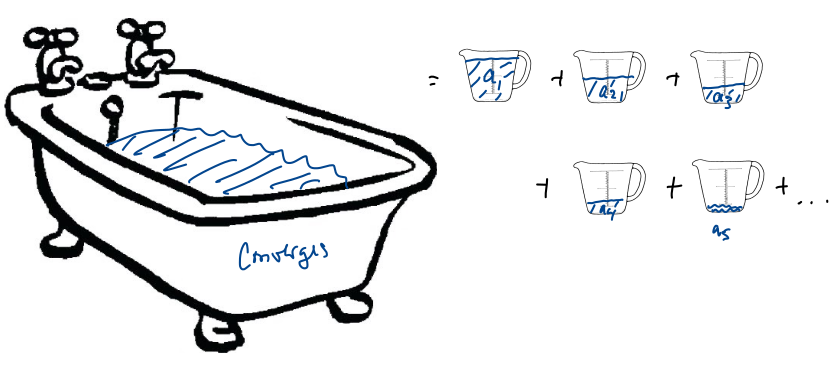
\includegraphics[width=.9\columnwidth]{Ch8s2-bath-conv.png}
\caption{Illustration of the convergent series bathtub analogy for Theorem 8.2.6}
\end{figure}


\subsection*{Theorem 8.2.6:}
If the series \(\Sum a_n\) is convergent, then \(\lim_{n\rightarrow\infty} a_n = 0\).

%\columnbreak

If the amount of water we add each time doesn't go to zero, then the bathtub will definitely overflow:\\

\begin{figure}[h]
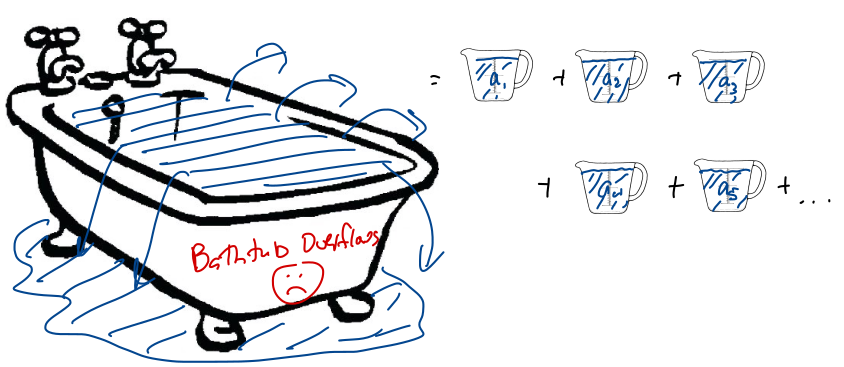
\includegraphics[width=.9\columnwidth]{Ch8s2-bath-div.png}
\caption{Illustration of the bathtub analogy for the Test for Divergence.}
\end{figure}

\subsection*{Test for Divergence:}
If \(\lim_{n\rightarrow\infty} a_n\) DNE \textbf{-OR-} \(\lim_{n\rightarrow\infty} a_n \neq 0\), then \(\Sum a_n\) is  divergent.\\~\\~\\

%\end{multicols}

%\hrule
\vspace*{.1in}

%\begin{multicols}{2}

\subsection*{Theorem 8.2.8: }

%\textbf{Theorem 8.2.6:}\\~\\
%If the series \(\Sum a_n\) is convergent, then \(\lim_{n\rightarrow\infty} a_n = 0\).\\~\\~\\
%
%\textbf{Theorem 8.2.8:}\\~\\
If \(\sum a_n\) and \(\sum b_n\) are convergent series, then so are:
\begin{enumerate}[(i)]
\item \(\sum c a_n = c\sum a_n\)
\item \(\sum (a_n+ b_n) = \sum	a_n + \sum	b_n\)
\item \(\sum (a_n- b_n) = \sum	a_n - \sum	b_n\)
\end{enumerate}

%\columnbreak

\section*{Series whose Convergence Behavior we Know:}



\subsection*{Geometric Series:}
\[ \sum_{n=1}^\infty a r^{n-1} = a+ ar+ ar^2+ ar^3+ \ldots+ ar^{n-1}+\ldots \]
\textbf{converges} to \(S=\frac{a}{1-r}\) if \(|r|<1\)\\
 \textbf{diverges} if \(|r|\geq 1\).\\

\vspace*{.1in}
%\hrule
\vspace*{.2in}

\subsection*{Harmonic Series:} 
\[ \sum_{n=1}^\infty \frac{1}{n} = 1+\frac{1}{2}+\frac{1}{3}+\frac{1}{4}+\frac{1}{5}+\ldots \]
\textbf{diverges}

%\end{multicols}

%%\hrule
%\vspace*{.2in}

%\df{\textcolor{sblack}{Test for Divergence:}}~\\
%If \(\lim_{n\rightarrow\infty} a_n\) DNE \textbf{-OR-} \(\lim_{n\rightarrow\infty} a_n \neq 0\), then \(\Sum a_n\) is  divergent.\\~\\~\\

%\end{framed}

%\end{minipage}

\pagebreak

\section*{Problems for Group Work:}
\textbf{Be sure to fully justify your reasoning as a part of your solutions.}\\
 The answers are upside-down on the bottom of this page.

\begin{enumerate}

\item Determine the convergence/divergence of the following series: \label{prob3}
\begin{enumerate}[a)]

\item \(\sum_{n=1}^\infty \ \frac{1}{k^n}, \quad k>1\)\vfill

\item \(\sum_{n=1}^\infty \ \frac{4\cdot 5^n - 5\cdot 4^n}{6^n}\)\vfill

\item \(\sum_{n=1}^\infty \ (-1)^n\)\vfill

\item \(\sum_{n=1}^\infty \ \sin\left(\frac{n}{n+1}\right)\)\vfill

\item \(\sum_{n=1}^\infty \ (-1)^{2n}\)\vfill

%\item \(\sum_{n=1}^\infty \ \left[\frac{5}{n(n+1)}-\left(-\frac{1}{2}\right)^n\right]\)\vfill

\end{enumerate}
%Solution: a) Converge, b) Converge, c) Diverge, d) Diverge, e) Diverge, f) Converge


%\item If the improper integral \(\int_5^\infty \frac{dx}{x^p}\) converges, which of the following series \underline{must} converge?\label{prob4}
%%\begin{multicols}{3}
%\begin{enumerate}[A)]
%\item \(\sum_{n=1}^\infty \ \frac{1}{n^{p+1}}\)
%
%\item \(\sum_{n=5}^\infty \ \frac{1}{n^{p+1}}\)
%
%\item \(\sum_{n=1}^\infty \ \frac{1}{n^{p-1}}\)
%
%\item \(\sum_{n=5}^\infty \ \frac{1}{n^{p-1}}\)
%
%\item Both A and B
%
%\item Both C and D
%
%\end{enumerate}
%%\end{multicols}


\end{enumerate}

\vfill

%\rotatebox{180}{
%\begin{minipage}{\textwidth}
\subsection*{Answers:}
%\textbf{Problem \ref{prob1}:} a) Diverge, b) Converge to 4, 
%\textbf{Problem \ref{prob2}:} a) Converges to \(\frac{3}{8}\), b) Converges to \(\frac{3}{\pi(\pi-3)}\), 
\textbf{Problem \ref{prob3}:} a) Converge, b) Converge, c) Diverge, d) Diverge, e) Diverge, %f) Converge, 
%\textbf{Problem \ref{prob4}:} E,
%\end{minipage}
%}

\end{document}
